\documentclass{beamer}
\usetheme{metropolis}
\usepackage{graphicx}
\usepackage{subfig}
\title{Algebra-Based Physics-1: Mechanics (PHYS135A-01): Week 1}
\date{September 6th - September 8th, 2017}
\author{Jordan Hanson}
\institute{Whittier College Department of Physics and Astronomy}

\begin{document}
\maketitle

\begin{frame}{Course Introduction}
\begin{enumerate}
\item Professor Jordan Hanson
\item Contact: jhanson2@whittier.edu, SLC 212
\item Syllabus: Moodle
\item Office hours: Tuesdays 12:50, Wednesdays 15:00
\item Text: College Physics (openstax.org)
\item Homework: Assigned from the book Mondays, due the following Monday
\item Lab notebooks (will distribute shortly)
\end{enumerate}
\end{frame}

\section{Opening Remarks - Welcome!}

\section{Course Introduction}

\begin{frame}{Course Introduction}
\begin{itemize}
\item What do you hope to learn from this course?
\item What do you hope to do with this new knowledge?
\item What do you expect the lectures to do for you?
\item What do you expect the book to do for you?
\item How many hours per week do you expect to spend on this course in order to have success?
\end{itemize}
\end{frame}

\section{Force and Motion and Conceptual Evaluation (FMCE)}

\begin{frame}{Week 1 Summary}
\textit{Physics} - $\phi\upsilon\sigma\iota\kappa\acute{\eta}$ - "phusik\'e": \textit{knowledge of nature} \\
from $\phi\acute{\upsilon}\sigma\iota\varsigma$ - "ph\'usis": \textit{nature}
\begin{enumerate}
\item Methods of approximation
\begin{itemize}
\item \alert{Estimating} the correct order of magnitude
\item \alert{Function} approximation
\item \alert{Unit analysis}
\end{itemize}
\item Coordinates and vectors
\begin{itemize}
\item \alert{Scalars} and \alert{vectors}
\item \alert{Cartesian} (rectangular) coordinates, displacement
\item \alert{Vector} addition, subtraction, and multiplication
\end{itemize}
\item Review of geometry and trigonometry techniques
\begin{itemize}
\item Similar triangles
\item Pythagorean theorem
\item Sine, cosine, tangent ...
\end{itemize}
\end{enumerate}
\end{frame}

\begin{frame}{Homework problems (Due Wednesday, September 13)}
\begin{itemize}
\item Chapter 1, exercise 1
\item Chapter 1, exercise 9
\item Chapter 1, exercise 10
\item Chapter 1, exercise 29
\item Chapter 1, exercise 35
\end{itemize}
\end{frame}

\section{Methods of approximation}

\begin{frame}{Methods of approximation - Estimation (Chapter 1)}
In science and engineering, \alert{estimation} is to obtain a quantity in the absence of precision, informed by rational constraints.
\begin{enumerate}
\item Define relevant \alert{scales}
\begin{itemize}
\item 1 \textit{AU} for the solar system (distance from Sun to Earth)
\item 1 \textit{angstrom} ($10^{-10}$ meters) for cell membranes
\end{itemize}
\item Obtain \alert{complex quantities} from simple ones
\begin{itemize}
\item Obtain \textit{areas} and \textit{volumes} from \textit{lengths}
\item Obtain \textit{rates} from \textit{numerators} and \textit{denominators}
\end{itemize}
\item Constrain the unknown with \alert{upper} and \alert{lower} limits
\begin{itemize}
\item The solar system is \textit{less than one light-year across}
\item An insect is \textit{at least one millimeter} long
\end{itemize}
\end{enumerate}
\end{frame}

\begin{frame}{Methods of approximation - Estimation (Chapter 1)}
\small
\begin{minipage}[b]{0.45\linewidth}
Estimate the mass of ants in an ant colony.  Assume that the colony is a species known to have $10^5$ ants (roughly) per colony.
\begin{itemize}
\item A: 0.01 kg
\item B: 0.1 kg
\item C: 1 kg
\item D: 10 kg
\end{itemize}
\end{minipage}
\hspace{0.5cm}
\begin{minipage}[b]{0.45\linewidth}
An adult blue whale is about 30 meters long.  What is the mass of a blue whale calf? (1 tonne = 1000 kg).
\vspace{0.55cm}
\begin{itemize}
\item A: 100 kg
\item B: 0.5 tonnes
\item C: 5 tonnes
\item D: 20 tonnes
\end{itemize}
\end{minipage}
\end{frame}

\begin{frame}{Methods of approximation - Estimation (Chapter 1)}
\begin{figure}
\centering
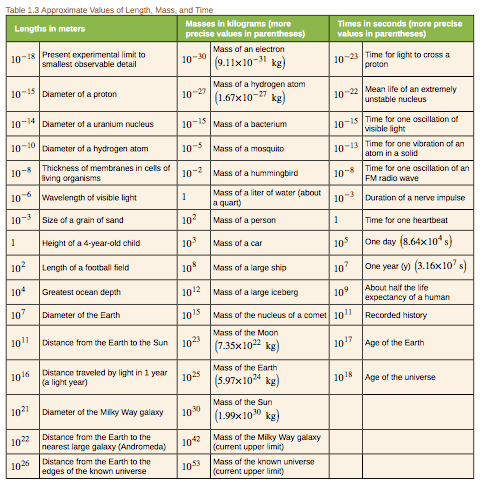
\includegraphics[width=0.6\textwidth]{figures/tab1.png}
\caption{\label{fig:tab1} Table 1.3 from the text.}
\end{figure}
\end{frame}

\begin{frame}{Methods of approximation - Estimation (Chapter 1)}
\small
\begin{minipage}[b]{0.45\linewidth}
How long does it take an airliner to fly across the Atlantic ocean?  Assume the velocity is 500 mph, and the radius of the Earth is 7000 km.
\vspace{0.6cm}
\begin{itemize}
\item A: 10 hours
\item B: 15 hours
\item C: 2 hours
\item D: 4 hours
\end{itemize}
\end{minipage}
\hspace{0.5cm}
\begin{minipage}[b]{0.45\linewidth}
A flock of birds takes one minute to pass overhead, and it is about 100 meters wide, with most birds flying at roughly the same altitude.  How many birds are in the flock?
\vspace{0.1cm}
\begin{itemize}
\item A: 100 birds
\item B: 1,000 birds
\item C: 10,000 birds
\item D: 100,000 birds
\end{itemize}
\end{minipage}
\end{frame}

\begin{frame}{Methods of approximation - Function approximation}
In science and engineering, \alert{function approximation} or \alert{expanding a function} is a technique in which a simple function is used obtain the value of a more complicated function near a point where they are approximately equal. 
\begin{enumerate}
\item Memorizing \alert{special cases}
\begin{itemize}
\item $\sin(x) \approx x$, when $|x| < 1$
\item $\tan(x) \approx x$, when $|x| < 1$
\item $(1+x)^{1/2} \approx 1+ \frac{1}{2}x$, when $|x| < 1$
\item $\exp(x) \approx 1 + x$, when $|x| < 1$
\end{itemize}
\item Utilizing the \textbf{Taylor Series} (encounter in calculus...)
\begin{itemize}
\item $f(x) \approx f(a) + \frac{f'(a)}{1!}(x-a) + \frac{f''(a)}{2!}(x-a)^2 + \frac{f'''(a)}{3!}(x-a)^3 + ...$
\end{itemize}
\end{enumerate}
\end{frame}

\begin{frame}{Methods of approximation - Function approximation}
\begin{figure}
\centering
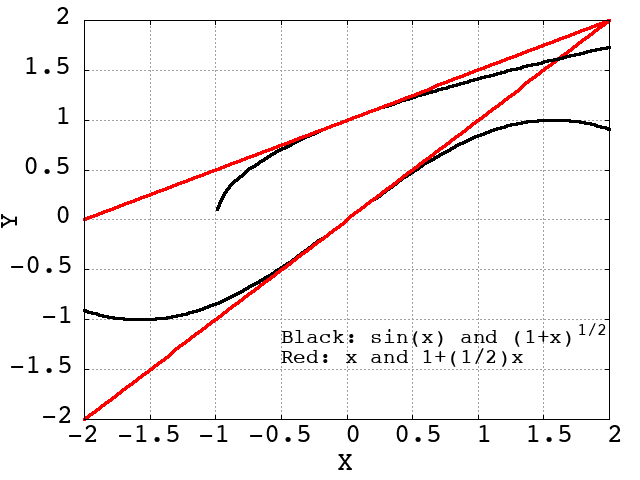
\includegraphics[width=0.7\textwidth]{figures/taylor_series.png}
\caption{\label{fig:approx} Certain functions may be approximated by simpler ones.  In this case, $\sin(x)$ is approximated by $x$ near $x=0$, and $(1+x)^{1/2}$ is approximated by $1+\frac{1}{2}x$ near $x=0$.}
\end{figure}
\end{frame}

\begin{frame}{Methods of approximation - Function approximation}
\small
\begin{minipage}[b]{0.45\linewidth}
The height in meters of a surfer above some average height as he bobs in the waves is described by $h(t) = sin(t)$.  What is his height at 1.0 second?  What is his height at -1.0 second?
\vspace{0.2cm}
\begin{itemize}
\item A: 1 meter, -1 meter
\item B: $\pi$ meters, -$\pi$ meters
\item C: -1 meter, 1 meter
\item D: -$\pi$ meters, $\pi$ meters
\end{itemize}
\end{minipage}
\hspace{0.5cm}
\begin{minipage}[b]{0.45\linewidth}
The value of an investment in dollars, $v$, versus time in years, $t$, follows the form $v(t) = P\exp(rt)$, where $P$ is the value at $t=0$, and $r=1/3$.  What is $v(1)$, the value after one year?
\vspace{0.6cm}
\begin{itemize}
\item A: $\approx 1/3 P$
\item B: $\approx 2/3 P$
\item C: $\approx 3/2 P$
\item D: $\approx 4/3 P$
\end{itemize}
\end{minipage}
\end{frame}

\begin{frame}{Methods of approximation - Units (Chapters 1)}
Physics requires \alert{units} to relate ideas to the real world, and \alert{unit analysis} is a powerful tool to eliminate incorrect results and to facilitate estimation.
\begin{enumerate}
\item SI units, and kilogram-meter-second unit set
\begin{itemize}
\item mass: \alert{kilogram} (gram = $10^{-3}$ kg, milligram = $10^{-6}$ kg)
\item length: \alert{meter} (millimeter = $10^{-3}$ m, kilometer = $10^{3}$ m)
\item time: \alert{second} (1 year $\approx \pi \times 10^{7}$ sec, 1 hour = 3600 sec)
\end{itemize}
\item Unit analysis
\begin{itemize}
\item If we are calculating a density, the units should work out to be kg/m$^3$
\item Identifying the fundamental unit in a complex calculation often simplifies it (when done properly, this reveals the beauty of physics)
\end{itemize}
\end{enumerate}
\end{frame}

\begin{frame}{Methods of approximation - Units (Chapters 1)}
\small
\begin{minipage}[b]{0.45\linewidth}
A millenium is 1000 years.  If a glacier retreats at a pace of 10 cm per year, what is this rate in meters per millenium?
\vspace{0.2cm}
\begin{itemize}
\item A: 0.1 meter per millenium
\item B: 1 meter per millenium
\item C: 10 meters per millenium
\item D: 100 meters per millenium
\end{itemize}
\end{minipage}
\hspace{0.5cm}
\begin{minipage}[b]{0.45\linewidth}
Ice has a density of 0.917 grams per centimeter cubed.  What is this density in kilograms per meter cubed?
\vspace{1.1cm}
\begin{itemize}
\item A: 91.7 kg/m$^3$
\item B: 917 kg/m$^3$
\item C: 9170 kg/m$^3$
\item D: 9.17 kg/m$^3$
\end{itemize}
\end{minipage}
\end{frame}

\begin{frame}{Methods of approximation - Units (Chapters 1)}
\centering
Sometimes, the beauty of physics arrises from choosing the right unit. \\
\vspace{1cm}
\small
\boxed{http://joshworth.com/dev/pixelspace/pixelspace\_solarsystem.html} \\
\vspace{1cm}
\normalsize
The Sun in this ruler is at 0 km, and Jupiter is at about 780,000,000 km (good luck finding it).  Clearly, the kilometer is the wrong unit to choose for interplanetary distances.  What if we defined a new unit, the \alert{astronomical unit}, as the distance between the Earth and the Sun?
\end{frame}

\begin{frame}{Methods of approximation - Units (Chapters 1)}
Planetary orbital radii in \alert{AU} (geometric means):
\begin{figure}
\begin{tabular}{| c | c |}
\hline
Mercury & 0.379 \\
Venus & 0.722 \\
Earth & 1.00 \\
Mars & 1.52 \\
Jupiter & 5.20 \\
Saturn & 9.54 \\
Uranus & 19.2 \\
Neptune & 30.1 \\
\hline
\end{tabular}
\caption{\label{tab:planets} Why such simple numbers?  There is a set of simple relationships between the \textit{orbital period} and the \textit{orbital radius} of planets called Kepler's Laws, which led to the discovery of \alert{Newton's Law of Gravity.}}
\end{figure}
\end{frame}

\section{Coordinates and Vectors}

\begin{frame}{Coordinates and Vectors - Scalars, Vectors (Chapters 2.1-2.2)}
Physics requires \alert{mathematical objects} to build equations that capture the behavior of nature.  Two examples of such objects are \alert{scalar} and \alert{vector} quantities.  Each type of object obeys similar but different rules.
\begin{enumerate}
\item Scalar quantities
\begin{itemize}
\item mass: $m_1+(m_2+m_3) = (m_1+m_2)+m_3$
\item speed: $v_1(v_2+v_3) = v_1v_2+v_1v_3$
\item charge: $q_1 \left(\frac{1}{q_1}\right) = 1$, $q_1(0) = 0$
\end{itemize}
\item Vector quantities
\begin{itemize}
\item velocity: $\vec{v}_1 + (\vec{v}_2+\vec{v}_3) = (\vec{v}_1 + \vec{v}_2)+\vec{v}_3$
\item tension: $\vec{t}_1 \cdot (\vec{t}_2 + \vec{t}_3) = \vec{t}_1 \cdot \vec{t}_2 + \vec{t}_1 \cdot \vec{t}_3$
\end{itemize}
\end{enumerate}
\end{frame}

\begin{frame}{Coordinates and Vectors - Scalars, Vectors (Chapters 2.1-2.2)}
A vector may be expressed as \textit{a list of scalars}: $\vec{v} = (4,2)$ (a vector with two \textit{components}), $\vec{u} = (3,4,5)$ (three \textit{components}).  Now, we know how to add and subtract scalars.  How do we add and subtract vectors? \\
\vspace{0.5cm}
What is\\
$(1,3,8)+$\\ $(0,2,1)$? \\
Answer: $(1,5,9)$ \\
\vspace{0.5cm}
In other words, when adding vectors, we add them component by component.
\end{frame}

\begin{frame}{Coordinates and Vectors - Scalars, Vectors (Chapters 2.1-2.2)}
How do we subtract vectors? In the same fashion:\\
\vspace{0.5cm}
What is\\
$(1,3,8)-$\\ $(0,2,1)$? \\
Answer: $(1,1,7)$ \\
\vspace{0.5cm}
In other words, when subtracting vectors, we subtract them component by component.
\end{frame}

\begin{frame}{Coordinates and Vectors - Scalars, Vectors (Chapters 2.1-2.2)}
How do we multiply vectors? In the same fashion, \textit{for one kind of multiplication}:\\
\vspace{0.5cm}
What is\\
$(1,3,8)\cdot (0,2,1)$? \\
Answer: $1\cdot 0 + 3 \cdot 2 + 8 \cdot 1 = 14$ \\
\vspace{0.5cm}
\textit{This kind of multiplication is known as the dot-product}.  There is also the \textit{cross-product}, which we will save for later.
\end{frame}

\begin{frame}{Coordinates and Vectors - Coordinates (Chapters 2.1-2.2)}
\small
The components of a vector may describe quantities in a \alert{coordinate system}, such as \textit{Cartesian coordinates} - after Ren\'e Descartes.  Vectors in the 3D Cartesian coordinate system (x,y,z) may be written in the following notation:
\\
\vspace{0.2cm}
$\boxed{\vec{v} = a\hat{i} + b\hat{j} + c\hat{k}}$
\\
\begin{itemize}
\item a: The amount in the +x-direction, $\hat{i}$: a vector of length 1, in the +x-direction
\item b: The amount in the +y-direction, $\hat{j}$: a vector of length 1, in the +y-direction
\item c: The amount in the +z-direction, $\hat{k}$: a vector of length 1, in the +z-direction
\end{itemize}
\end{frame}

\begin{frame}{Coordinates and Vectors - Vectors (Chapters 2.1-2.2)}
\begin{figure}
\centering
\subfloat[\label{fig:twovectors_a}]{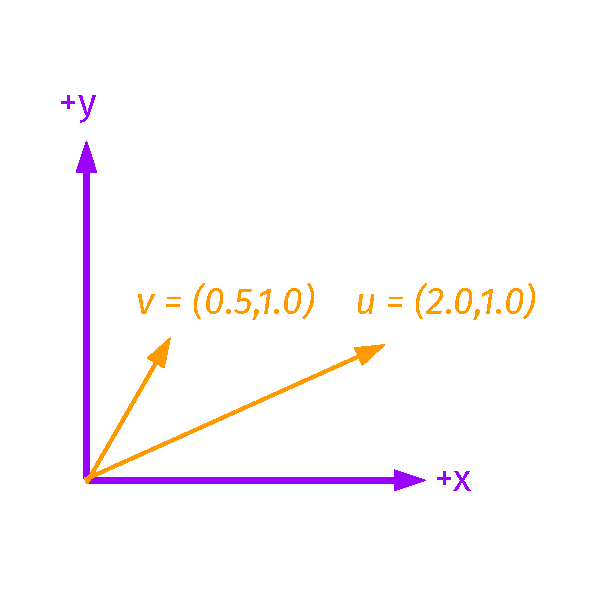
\includegraphics[width=0.45\textwidth,trim=1cm 1cm 1cm 1cm,clip=true]{figures/Vectors1.pdf}}
\subfloat[\label{fig:twovectors_b}]{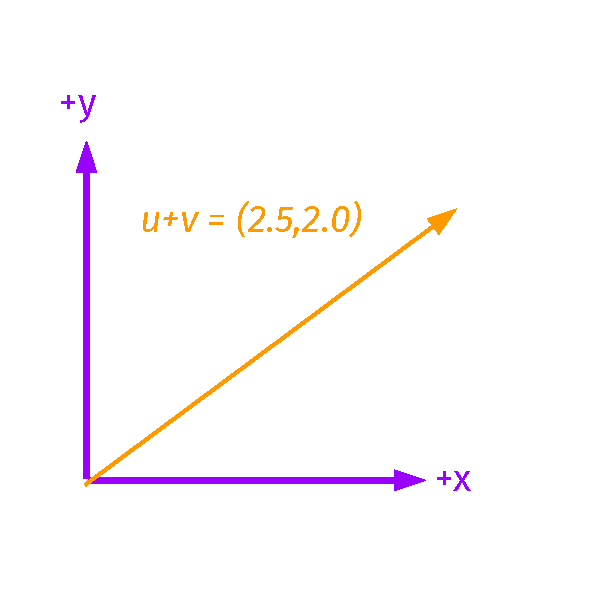
\includegraphics[width=0.45\textwidth,trim=1cm 1cm 1cm 1cm,clip=true]{figures/Vectors2.pdf}}
\caption{\label{fig:twovectors} (a) Two vectors in a two-dimensional Cartesian coordinate system: $\vec{u} = 0.5\hat{i}+1.0\hat{j}$ and $\vec{v} = 2.0\hat{i}+1.0\hat{j}$.  (b) What is $\vec{u}+\vec{v}$?  Adding components: $\vec{u}+\vec{v} = 2.5\hat{i}+2.0\hat{j}$.}
\end{figure}
\end{frame}

\begin{frame}{Coordinates and Vectors - Vectors (Chapters 2.1-2.2)}
\begin{figure}
\centering
\subfloat[\label{fig:twovectors_c}]{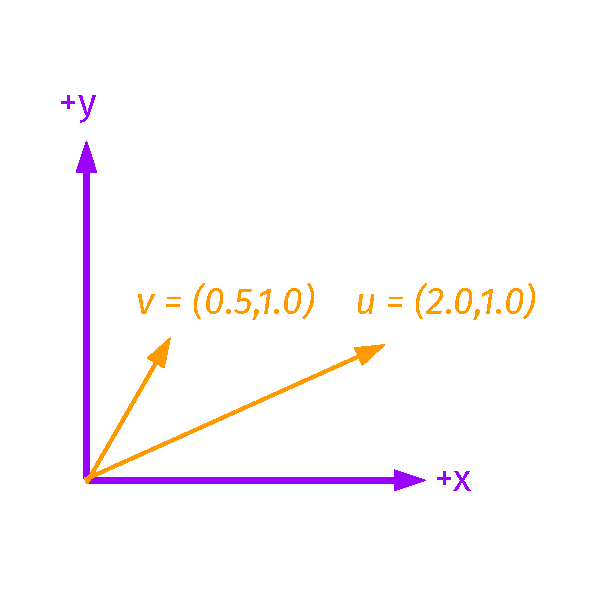
\includegraphics[width=0.45\textwidth,trim=1cm 1cm 1cm 1cm,clip=true]{figures/Vectors1.pdf}}
\subfloat[\label{fig:twovectors_d}]{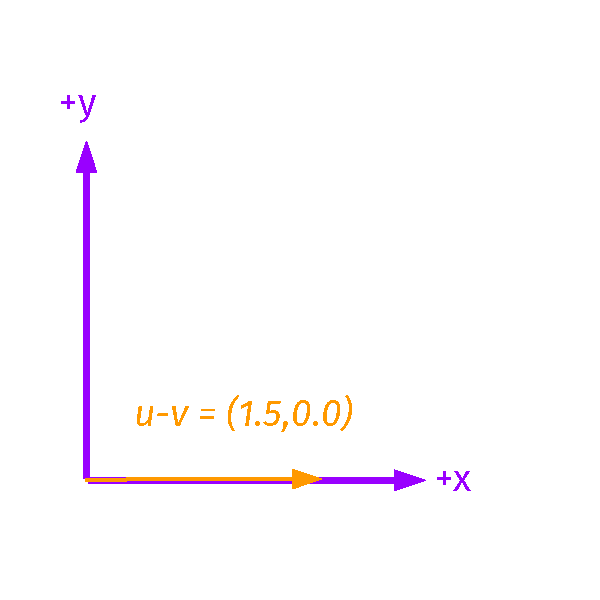
\includegraphics[width=0.45\textwidth,trim=1cm 1cm 1cm 1cm,clip=true]{figures/Vectors3.pdf}}
\caption{\label{fig:twovectors2} (a) Two vectors in a two-dimensional Cartesian coordinate system: $\vec{u} = 0.5\hat{i}+1.0\hat{j}$ and $\vec{v} = 2.0\hat{i}+1.0\hat{j}$.  (b) What is $\vec{u}-\vec{v}$?  Subtracting components: $\vec{u}-\vec{v} = 1.5\hat{i}+0.0\hat{j}$.}
\end{figure}
\end{frame}

\begin{frame}{Coordinates and Vectors - Vectors (Chapters 2.1-2.2)}
\begin{figure}
\centering
\subfloat[\label{fig:twovectors_e}]{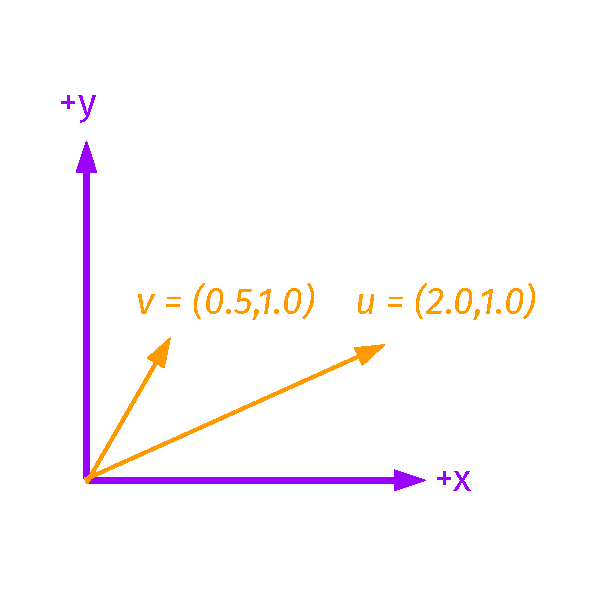
\includegraphics[width=0.45\textwidth,trim=1cm 1cm 1cm 1cm,clip=true]{figures/Vectors1.pdf}}
\subfloat[\label{fig:twovectors_f}]{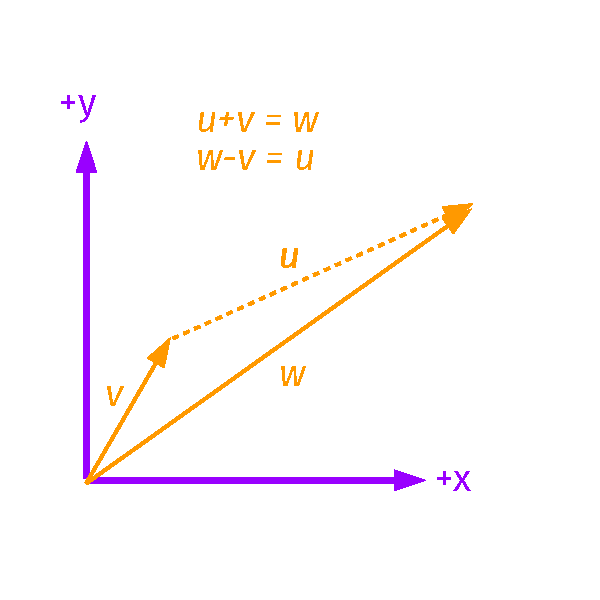
\includegraphics[width=0.45\textwidth,trim=1cm 1cm 1cm 1cm,clip=true]{figures/Vectors4.pdf}}
\caption{\label{fig:twovectors3} (a) Two vectors in a two-dimensional Cartesian coordinate system: $\vec{u} = 0.5\hat{i}+1.0\hat{j}$ and $\vec{v} = 2.0\hat{i}+1.0\hat{j}$.  (b) To compute $\vec{w}-\vec{v}$, arrange the vectors to get a sense of the result, $\vec{u}$.}
\end{figure}
\end{frame}

\begin{frame}{Coordinates and Vectors - Vectors (Chapters 2.1-2.2)}
\small
\begin{minipage}[b]{0.45\linewidth}
$\vec{p} = 4\hat{i}+2\hat{j}$.  $\vec{q} = -4\hat{i}+2\hat{j}$.  \\
Compute $\vec{p} \cdot \vec{q}$.
\vspace{0.2cm}
\begin{itemize}
\item A: 12
\item B: -12
\item C: 4
\item D: 8
\end{itemize}
\end{minipage}
\hspace{0.5cm}
\begin{minipage}[b]{0.45\linewidth}
$\vec{p} = -1\hat{i}+6\hat{j}$.  $\vec{q} = 3\hat{i}+0.5\hat{j}$.  \\
Compute $\vec{p} \cdot \vec{q}$.
\vspace{0.2cm}
\begin{itemize}
\item A: -1
\item B: 1
\item C: 0
\item D: 3
\end{itemize}
\end{minipage}
\end{frame}

\begin{frame}{Coordinates and Vectors - Vectors (Chapters 2.1-2.2)}
Why was the last answer zero?  Look at it graphically:
\begin{figure}
\centering
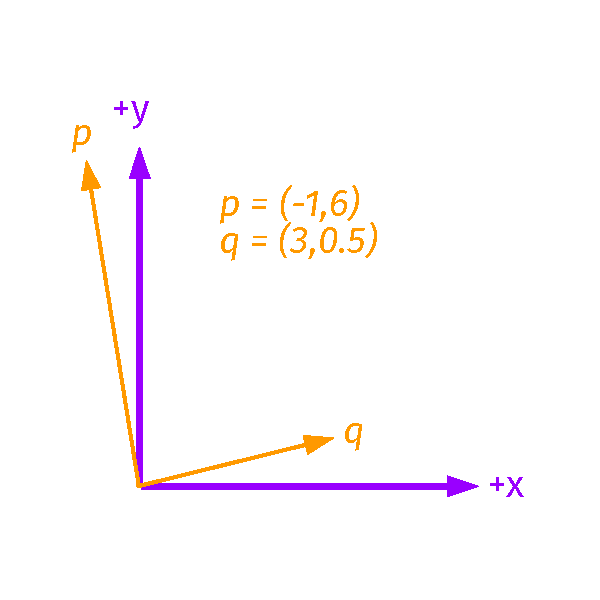
\includegraphics[width=0.5\textwidth,trim=1cm 1cm 1cm 1cm,clip=true]{figures/Vectors5.pdf}
\caption{\label{fig:twovectors4} Two vectors $\vec{p}$ and $\vec{q}$ are \textit{orthogonal} if $\vec{p} \cdot \vec{q} = 0$.}
\end{figure}
\end{frame}

\begin{frame}{Coordinates and Vectors - Vectors (Chapters 2.1-2.2)}
What if the vectors are parallel? Look at it graphically:
\begin{figure}
\centering
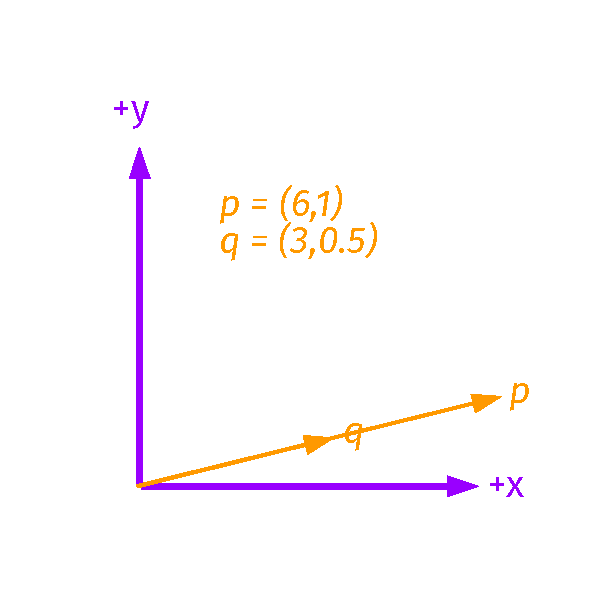
\includegraphics[width=0.5\textwidth,trim=1cm 1cm 1cm 1cm,clip=true]{figures/Vectors6.pdf}
\caption{\label{fig:twovectors5} Two vectors $\vec{p}$ and $\vec{q}$ are \textit{parallel} if $\vec{p} \cdot \vec{q}$ is maximal.}
\end{figure}
\end{frame}

\begin{frame}{Coordinates and Vectors - Dot Product (Chapters 2.1-2.2)}
The \textit{length} or \textit{norm} of a vector $\vec{v} = a\hat{i}+b\hat{j}$ is $|\vec{v}| = \sqrt{a^2+b^2}$.\\
\begin{figure}
\centering
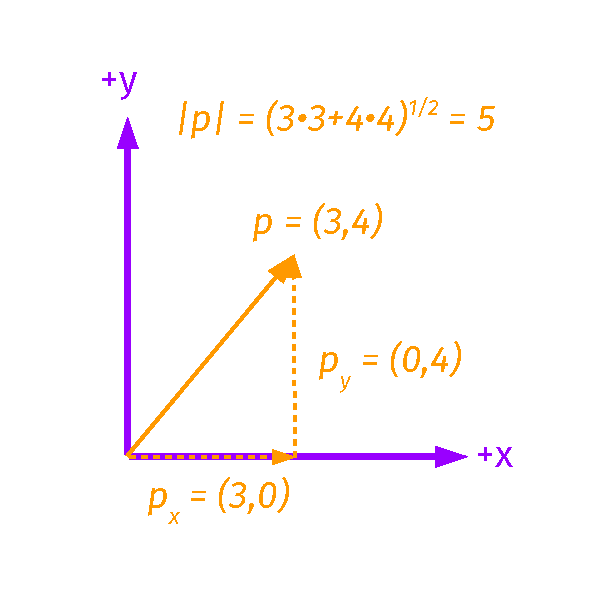
\includegraphics[width=0.5\textwidth,trim=1cm 1cm 1cm 1cm,clip=true]{figures/Vectors7.pdf}
\caption{\label{fig:twovectors6} Computing the norm of a vector $\vec{p}$.}
\end{figure}
\end{frame}

\begin{frame}{Coordinates and Vectors - Dot Product (Chapters 2.1-2.2)}
Notice that $\sqrt{\vec{p}\cdot\vec{p}} = |\vec{p}|$.\\
Let $\theta_p$ be the angle between $\vec{p}$ and the x-axis.  \\
$p_{x} = \vec{p} \cdot \hat{i} = |\vec{p}| \cos(\theta_{p})$. \\
$p_{y} = \vec{p} \cdot \hat{j} = |\vec{p}| \sin(\theta_{p})$.\\
\vspace{0.5cm}
\textit{Theorem:} The dot product of two vectors $\vec{p}$ and $\vec{q}$ is $|u||v|\cos(\theta)$, if $\theta$ is the angle between them.\\
\vspace{0.5cm}
\textit{Proof}: $\vec{p}\cdot\vec{q} = p_{x}q_{x} + p_{y}q_{y} = |p||q|\cos\theta_p\cos\theta_q+|p||q|\sin\theta_q\sin\theta_q$ \\
$=|p||q|(\cos\theta_p\cos\theta_q+\sin\theta_p\sin\theta_q) = |p||q|\cos(\theta_p-\theta_q)$ \\
$=|p||q|\cos\theta$. \\
\vspace{0.1cm}
$\boxed{\vec{p}\cdot\vec{q}=|p||q|\cos\theta}$
\end{frame}

\begin{frame}{Coordinates and Vectors - Dot Product (Chapters 2.1-2.2)}
\small
\begin{minipage}[b]{0.45\linewidth}
An object moves at 2 m/s at $\theta = 60^{\circ}$ with respect to the x-axis.  What is the velocity of the object?
\vspace{0.2cm}
\begin{itemize}
\item A: $(1\hat{i}$ + $1\hat{j})$  m/s
\item B: $(\sqrt{3}\hat{i}$ + $1\hat{j})$  m/s
\item C: $(\sqrt{3}\hat{i}$ + $\sqrt{3}\hat{j})$  m/s
\item D: $(1\hat{i}$ + $\sqrt{3}\hat{j})$  m/s
\end{itemize}
\end{minipage}
\hspace{0.5cm}
\begin{minipage}[b]{0.45\linewidth}
What is the dot product of this velocity with another velocity: 5 m/s along the x-axis?
\vspace{0.7cm}
\begin{itemize}
\item A: 1 (m/s)$^2$
\item B: 5 (m/s)$^2$
\item C: 10 (m/s)$^2$
\item D: 5 (m/s)
\end{itemize}
\end{minipage}
\end{frame}

\begin{frame}{Coordinates and Vectors - Scalars, Vectors (Chapters 2.1-2.2)}
Is it possible to multiply vectors and scalars?  Of course: $a_1\vec{p} = a_1p_x\hat{i}+a_1p_y\hat{j}$.\\
\vspace{0.2cm}
Also, multiplication properties still hold.  For example: $(a_1+a_2)\vec{p} = a_1\vec{p}+a_2\vec{p}$. \\
\vspace{0.2cm}
\small
A spacecraft moves at 400 m/s, at an angle of 30 degrees with respect to the x-axis.  If it fires two thrusters that boost the x-component and y-component of the velocity by 25\% and 50\%, respectively, what is the final velocity?
\begin{itemize}
\item A: $(433\hat{i}+300\hat{j})$ m/s
\item B: $(300\hat{i}+433\hat{j})$ m/s
\item C: 400 m/s
\item D: $(400\hat{i}+433\hat{j})$ m/s
\end{itemize}
\end{frame}

\begin{frame}{Coordinates and Vectors - Dislacement (Chapters 2.1-2.2)}
We define the \textit{position} of an object as a vector locating it in a given coordinate system.  The scalar \textit{distance} is the norm of the position vector, that is, the distance to to the origin. \\
\vspace{0.5cm}
Now we can introduce the concept of \alert{dislacement}: a vector describing a movement of an object.
\end{frame}

\begin{frame}{Coordinates and Vectors - Displacement (Chapters 2.1-2.2)}
\begin{figure}
\centering
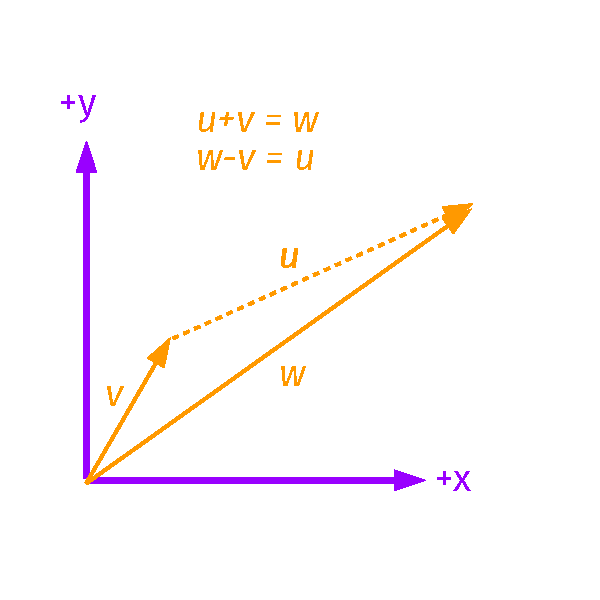
\includegraphics[width=0.52\textwidth]{figures/Vectors4.pdf}
\caption{\label{fig:displacement} Suppose an object moves from position $\vec{v}$ to $\vec{w}$.  In this case, the \alert{displacement} is $\vec{u}$. \textbf{Thus, the final position is the initial position, plus the displacement.}}
\end{figure}
\end{frame}

\begin{frame}{Coordinates and Vectors - Displacement (Chapters 2.1-2.2)}
It follows that the \textit{displacement} is zero if the initial and final positions are the same, but the \textit{distance travelled} is not.\\
\vspace{0.2cm}
\small
Suppose a jet fighter travelling at 800 km per hour banks such that it flies in a circle of radius 0.5 km.  How long does it take to complete the circle?  What is the distance traveled, and what is the displacement?
\begin{itemize}
\item A: $2\pi$ km, 28 seconds, $2\pi$ km
\item B: $\pi$ km, 14 seconds, $\pi$ km
\item C: $\pi$ km, 28 seconds, $\pi$ km
\item D: $\pi$ km, 14 seconds, $0$ km
\end{itemize}
\end{frame}

\begin{frame}{Coordinates and Vectors - Applications: displacement}
Jet fighters in the film Top Gun (1986):
\url{https://www.youtube.com/watch?v=WhYZc08Jk_Y}
\end{frame}

\begin{frame}{Coordinates and Vectors - Computer demonstration}
Download the Java applet (you may need to update Java): \\
\url{https://phet.colorado.edu/en/simulation/vector-addition}
\end{frame}

\begin{frame}{Coordinates and Vectors - Simulation activity}
\small
Let the y-axis represent altitude, and the x-axis represent horizontal distance.  Let the distance unit at the top right (for $R_x$ and $R_y$) be 100 m.  That is, 5 corresponds to 500 m.
\begin{itemize}
\item Using the vector tool, create a displacement vector for Jester's jet fighter.
\begin{enumerate}
\item Jester begins the dive at 3 km altitude and ends at 1 km.
\item He begins at a horizontal distance of 0 km, and the angle of his dive is -45 degrees.
\end{enumerate}
\item Using the vector tool, create a displacement vector for Maverick's jet fighter.
\begin{enumerate}
\item Maverick begins the dive at 2.5 km and ends at 1 km.
\item He begins at a horizontal distance of 0 km, and the angle of his dive is -45 degrees.
\end{enumerate}
\end{itemize}
\end{frame}

\begin{frame}{Coordinates and Vectors - Simulation activity}
\small
Let the y-axis represent altitude, and the x-axis represent horizontal distance.  Let the distance unit at the top right (for $R_x$ and $R_y$) be 100 m.  That is, 5 corresponds to 500 m.
\begin{itemize}
\item What is the initial displacement vector between Maverick and Jester? (Take Jester's initial position and subtract Maverick's initial position).
\item What are the final positions of Jester and Maverick?  Specify both the x and y coordinates.
\item What distance does each jet fighter travel?
\item Suppose the speed of each aircraft is 0.1 km/s.  How long does the dive take?
\item Given that you know how long the dive takes, what is the velocity vector of the aircraft?  (It's the same for both fighters).
\end{itemize}
\end{frame}

\begin{frame}{Coordinates and Vectors - Average Velocity  (Chapter 2.3)}
\alert{Average velocity} is the ratio of the \alert{displacement} to the elapsed time.\\
\begin{equation}
\boxed{\vec{v}_{\rm avg} = \frac{\Delta \vec{x}}{\Delta t}}
\end{equation}
The \textit{average speed} is the norm of the average velocity:
\begin{equation}
\boxed{v_{\rm avg} = \frac{|\Delta \vec{x}|}{\Delta t}}
\end{equation}
If the motion is in one dimension, then the average speed is
\begin{equation}
v_{\rm avg} = \frac{x_{\rm f} - x_{\rm i}}{t_{\rm f} - t_{\rm i}}
\end{equation}
\end{frame}

\begin{frame}{Coordinates and Vectors - Average Velocity (Chapter 2.3)}
\begin{figure}
\centering
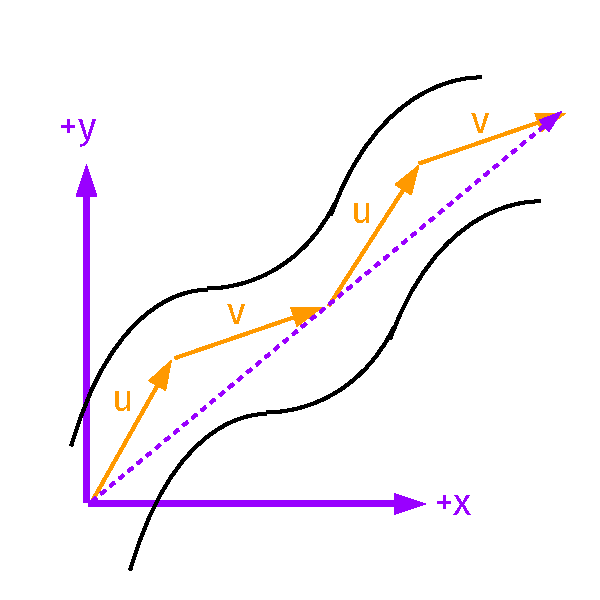
\includegraphics[width=0.52\textwidth]{figures/AveVelocity.pdf}
\caption{\label{fig:avevel} A Formula-1 driver keeps his car on the track by following a path approximated by the position vectors $u$, $v$, $u$, and $v$.  The dashed arrow represents the total displacement.}
\end{figure}
\end{frame}

\begin{frame}{Coordinates and Vectors - Average Velocity (Chapter 2.3)}
If $\vec{u} = (20\hat{i}+30\hat{j})$ m, and $\vec{v} = (30\hat{i}+20\hat{j})$ m, what is the total displacement?  If the elapsed time is 10 seconds, what is the average velocity? \\
\vspace{0.2cm}
\begin{itemize}
\item A: $(50\hat{i} + 50\hat{j})$ m, 14 m/s
\item B: $(80\hat{i} + 100\hat{j})$ m, 10 m/s
\item C: $(100\hat{i} + 100\hat{j})$ m, 14 m/s
\item D: $(50\hat{i} + 150\hat{j})$ m, 10 m/s
\end{itemize}
\end{frame}

\section{Review of Geometry and Trigonometry Techniques}

\begin{frame}{Review of Geometry and Trigonometry Techniques}
\small
\begin{figure}
\centering
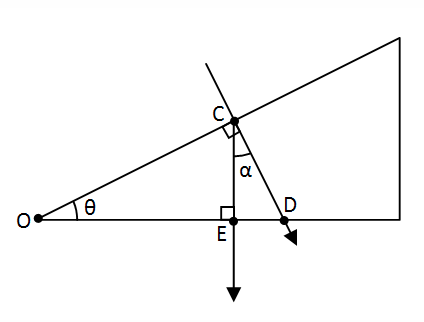
\includegraphics[width=0.4\textwidth]{figures/incline.png}
\caption{\label{fig:incline} Angles of a triangle add up to $\pi$ (180$^{\circ}$).}
\end{figure}
\begin{align}
\angle OCD &= \pi/2 = \angle OCE + \angle DCE = \angle OCE + \alpha \\
\angle OCE & + \angle COE + \pi/2 = \pi = \angle OCE + \theta + \pi/2 \\
\angle OCE &+ \theta = \pi/2 \\
\theta &= \alpha
\end{align}
\end{frame}

\begin{frame}{Review of Geometry and Trigonometry Techniques}
\small
\begin{figure}
\centering
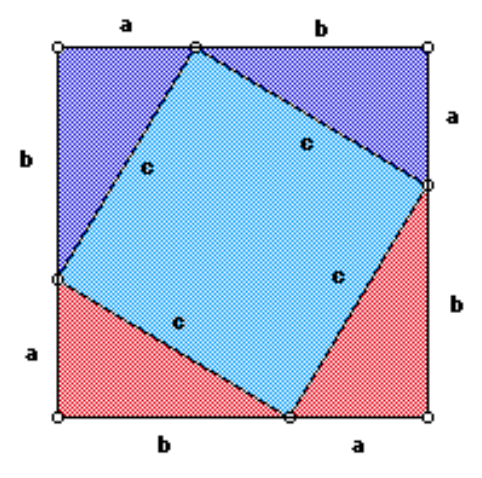
\includegraphics[width=0.4\textwidth]{figures/pyth.png}
\caption{\label{fig:pyth} Proof of Pythagorean theorem.}
\end{figure}
\begin{align}
A_1 &= (a+b)^2 = a^2 + b^2 + 4((1/2) a b) \\
A_2 &= c^2 + 4((1/2)ab) = A_1 \\
a^2 &+ b^2 = c^2
\end{align}
\end{frame}

\begin{frame}{Review of Geometry and Trigonometry Techniques}
One soccer teammate passes the ball to another.  The player without the ball is 7 meters away from the player with the ball, and they are both running in the same direction.  The player without the ball runs ahead by 24 meters before the pass.  How far does the ball travel? \\
\begin{itemize}
\item A: 7 meters
\item B: 24 meters
\item C: 25 meters
\item D: 17 meters
\end{itemize}
\end{frame}

\begin{frame}{Review of Geometry and Trigonometry Techniques}
\small
\begin{figure}
\centering
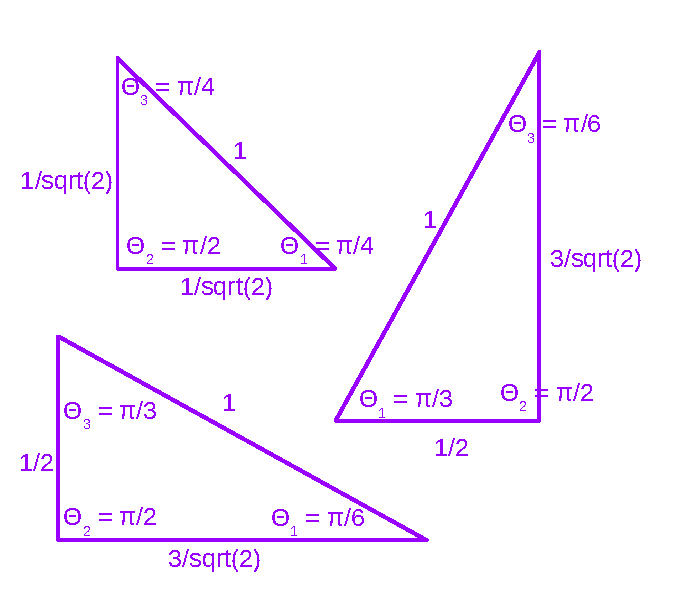
\includegraphics[width=0.6\textwidth]{figures/triangles.pdf}
\caption{\label{fig:triangles} \alert{Memorize} the properties of these special triangles.}
\end{figure}
\end{frame}

\begin{frame}{Review of Geometry and Trigonometry Techniques}
\small
\begin{figure}
\centering
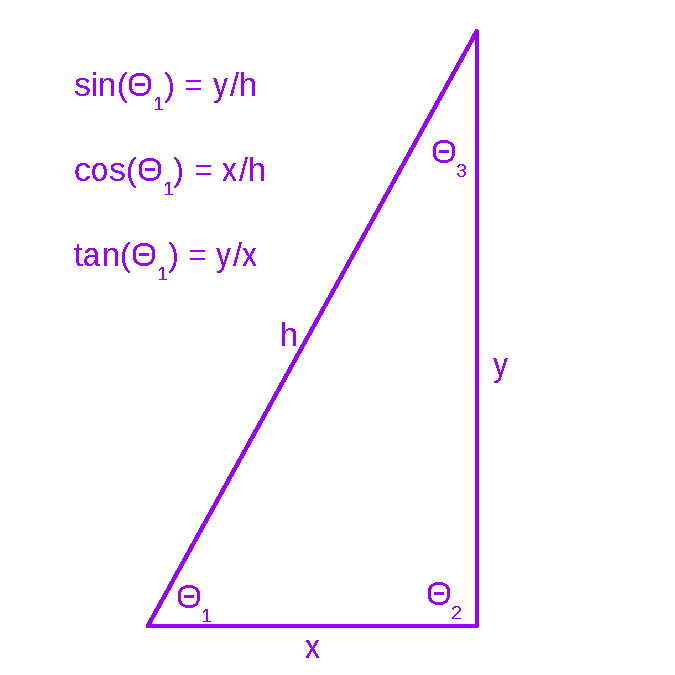
\includegraphics[width=0.6\textwidth]{figures/triangles2.pdf}
\caption{\label{fig:triangles2} Working definitions of trigonometric functions.}
\end{figure}
\end{frame}

\begin{frame}{Review of Geometry and Trigonometry Techniques}
\begin{columns}[T]
\begin{column}{0.5\textwidth}
What is $\sin(30^{\circ})$?
\begin{itemize}
\item A: 1/2
\item B: $\sqrt{3}/2$
\item C: 0
\item D: 1
\end{itemize}
\end{column}
\begin{column}{0.5\textwidth}
What is $\tan(45^{\circ})$?
\begin{itemize}
\item A: 1/2
\item B: $\sqrt{3}/2$
\item C: 0
\item D: 1
\end{itemize}
\end{column}
\end{columns}
\end{frame}

\begin{frame}{Review of Geometry and Trigonometry Techniques}
\small
\begin{columns}[T]
\begin{column}{0.4\textwidth}
What is $\sin(30^{\circ})^2+\cos(30^{\circ})^2$?
\begin{itemize}
\item A: 1/2
\item B: $\sqrt{3}/2$
\item C: 0
\item D: 1
\end{itemize}
\end{column}
\begin{column}{0.6\textwidth}
A right-triangle has sides of length 3, 4, and a hypoteneuse of 5.  What are the angles inside the triangle?
\begin{itemize}
\item A: $\arctan(5/4)$, $\arctan(4/5)$, $\pi/2$
\item B: $\arctan(1)$, $\arctan(4/5)$, $\pi/2$
\item C: $\arctan(4/3)$, $\arctan(3/4)$, $\pi/2$
\item D: $\arctan(3/4)$, $\arctan(3/4)$, $\pi/2$
\end{itemize}
\end{column}
\end{columns}
\end{frame}

\section{Conclusion}

\begin{frame}{Week 1 Summary}
\textbf{Chapters 1, 2}.
\begin{enumerate}
\item Methods of approximation
\begin{itemize}
\item \alert{Estimating} the correct order of magnitude
\item \alert{Function} approximation
\item \alert{Unit analysis}
\end{itemize}
\item Coordinates and vectors
\begin{itemize}
\item \alert{Scalars} and \alert{vectors}
\item \alert{Cartesian} (rectangular) coordinates, displacement
\item \alert{Vector} addition, subtraction, and multiplication
\end{itemize}
\item Review of geometry and trigonometry techniques
\begin{itemize}
\item Parallel lines, similar triangles
\item Pythagorean theorem
\item Sine, cosine, tangent ...
\end{itemize}
\end{enumerate}
\end{frame}

\section{Answers}

\begin{frame}{Answers}
\begin{columns}[T]
\begin{column}{0.5\textwidth}
\begin{itemize}
\item Mass of ants: 0.1 kg
\item Mass of baby whale: 5 tonnes
\item Length of flight is 10 hours
\item Number of birds is 10,000
\item Height of surfer is 1.0 meter, -1.0 meter
\item Value of investment is $4/3 P$
\item The glacier is retreating at 100 meters per millenium
\item Ice has a density of 917 kg/m$^3$
\end{itemize}
\end{column}
\begin{column}{0.5\textwidth}
\begin{itemize}
\item -12
\item 0
\item $(1\hat{i}$ + $\sqrt{3}\hat{j})$  m/s
\item 10 (m/s)$^2$
\item $(433\hat{i}+300\hat{j})$ m/s
\item $\pi$ km, 14 seconds, $0$ km
\item $(100\hat{i} + 100\hat{j})$ m, 14 m/s
\item 25 meters
\item 1/2
\item 1
\item $\arctan(4/3)$, $\arctan(3/4)$, $\pi/2$
\end{itemize}
\end{column}
\end{columns}
\end{frame}

\end{document}
